\documentclass[10pt]{beamer}
\usepackage{bbm}
\usepackage{fontspec}

\usepackage{algorithm2e}
\usepackage{mathtools}
\usepackage{graphicx}
\usepackage{animate}
\renewcommand\appendixname{Appendix}
\usepackage{xcolor}
\usepackage{tikz}
\colorlet{rred}{red!80!black}
\colorlet{ggreen}{green!80!black}
\colorlet{grey}{black!50!white}




\usetheme[progressbar=foot]{metropolis}
\usepackage{appendixnumberbeamer}
\setbeamercovered{dynamic}

\usepackage{booktabs}
\usepackage[scale=2]{ccicons}

\usepackage{pgfplots}
\usepgfplotslibrary{dateplot}
\setbeamertemplate{caption}{\raggedright\insertcaption\par}
\setlength{\abovecaptionskip}{-3pt plus 0pt minus 0pt}

\usepackage{xspace}
\newcommand{\themename}{\textbf{\textsc{metropolis}}\xspace}
\theoremstyle{definition}
\newtheorem{defn}{Definition}
\newtheorem{obs}{Observation}

% math symbols
\newcommand{\R}{\mathbb{R}}
\newcommand{\N}{\mathbb{N}}
\newcommand{\Z}{\mathbb{Z}}
\newcommand{\E}{\mathbb{E}}
\newcommand{\HBB}{\mathbb{H}}
\newcommand{\1}{\mathbbm{1}}
\newcommand{\XX}{\mathcal{X}}
\newcommand{\TT}{\mathcal{T}}
\newcommand{\YY}{\mathcal{Y}}
\newcommand{\UU}{\mathcal{U}}
\newcommand{\VV}{\mathcal{V}}
\newcommand{\WW}{\mathcal{W}}
\newcommand{\LL}{\mathcal{L}}
\newcommand{\PP}{\mathcal{P}}
\newcommand{\QQ}{\mathcal{Q}}
\DeclareMathOperator*{\argmin}{argmin}
\DeclareMathOperator*{\argmax}{argmax}
\title{An introduction to t-SNE}
\subtitle{Weekly AI pills}
\date{2020-11-13}
\author{Fabio Brau.}
\institute{SSSA, Emerging Digital Technologies, Pisa.}
% \titlegraphic{\hfill\includegraphics[height=1.5cm]{logo.pdf}}

\usebackgroundtemplate{%
    \begin{picture}(300,271)
      \hspace{11.2cm}
       
\includegraphics[scale=0.1]{pic/logoretis_noname.png}
   \end{picture}}

\begin{document}
{\usebackgroundtemplate{%
    \begin{picture}(300,265)
      \hspace{0.9cm}
       
\includegraphics[scale=0.5]{pic/tecip_logo.png}
       \hspace{0.5cm}
       
\includegraphics[scale=0.21]{pic/logoretis_320.png}
   \end{picture}}%
\maketitle
}
\begin{frame}{Summary}
  \tableofcontents
\end{frame}
\begin{frame}{Introduction}{}
%    \vfill
  \begin{center}
    (t)-{\bf S}tochastic {\bf N}eighborhood {\bf E}mbedding
  \end{center}
  \begin{minipage}{0.53\textwidth}
    {\bf Main Papers}
    \begin{itemize}
      \item Stochastic Neighbor Embedding - Hinton \& Roweis - 2002\\
      \item Visualizing Data using t-SNE - Maaten \& Hinton - 2008\\
    \end{itemize}
    \vspace{0.75cm}
    {\bf Aims}
    \begin{itemize}
      \item Dimensionality Reduction
      \item Data Visualization
        \begin{enumerate}
          \item Exploration
          \item Clusters Visualization
        \end{enumerate}
    \end{itemize}
  \end{minipage}\hfill
  \begin{minipage}{0.4\textwidth}
    \begin{figure}[h!]
      \centering
      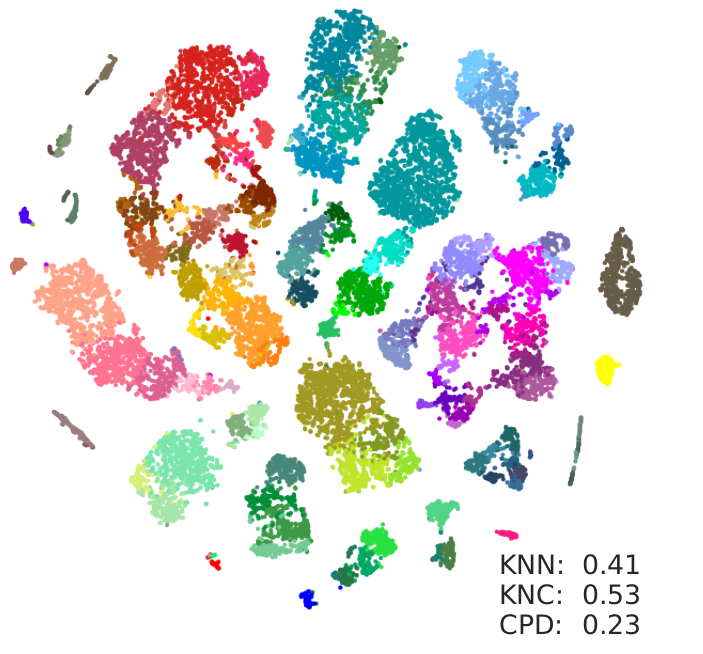
\includegraphics[scale=0.2]{./pic/example.png}
      \caption{Example of Data Visualization taken from (Tasic et al., 2018)}
    \end{figure}
  \end{minipage} 
\end{frame}
\section{SNE Algorithm}
\begin{frame}{SNE algorithm: Workflow}
  \begin{enumerate}
    \item Represent each sample $x_i \in\XX$ with $y_i\in\YY$ in a
      low-dimensional space
      \[
        \Phi :
        \underset{\subseteq \R^n}{\XX} \longrightarrow
        \underset{\subseteq \R^2}{\YY}
    \]
    \item Convert {\bf Geometrical Information} to {\bf Probabilistic
      Distribution} 
      \[
        \begin{aligned}
          p_{i|j} : \mbox{``Probability that $x_i$ is {\it\color{gray}
          similar} to $x_j$'' }\\
          q_{i|j} : \mbox{``Probability that $y_i$ is {\it\color{gray}
          similar} to $y_j$'' }
        \end{aligned}
      \]
    \item Compare distribution $\PP$ of $\XX$ to distribution $\QQ$ of $\XX$
    \item Adjust the representation $\Phi$ to make distributions closer.
  \end{enumerate}
  \onslide<2->
  \begin{obs}
    The embedding $\Phi$ is defined {\bf point-wise}, i.e $\Phi$ is only defined over
    $\XX$ through the definition $\Phi(x_i) = y_i$. Another way to say
    ``$y_i$ are the parameters of $\Phi$''.
  \end{obs}
\end{frame}
\begin{frame}{SNE algorithm: Similarity and Probability Distribution}
  \begin{defn}[Similarity with Gaussian Kernel]
    \vspace{1px}
    For each $x_i$ we consider the similarity
    \begin{equation}
      \forall j\ne i,\quad p_{i|j}  = \frac{\exp\left(-\|x_i -
      x_j\|^2/(2\sigma_i)^2\right)}{\sum_{k\ne i}\exp\left(-\|x_i - x_k\|^2 /
    (2\sigma_i)^2\right)}
      \tag{$\PP_i$}
    \end{equation}
    where $\sigma_i$ is an hyper-parameter depending on $x_i$.
  \end{defn}
  \onslide<2->
  {\bf How $\sigma_i$ impacts on $p_{i|j}$?}
  \begin{figure}[h!]
    \centering
    \includegraphics<2>[scale=0.4, trim=0 0 0 1cm]{{pic/similarity_0.1}.pdf}%
    \includegraphics<3>[scale=0.4, trim=0 0 0 1cm]{{pic/similarity_0.2}.pdf}%
    \includegraphics<4>[scale=0.4, trim=0 0 0 1cm]{{pic/similarity_0.5}.pdf}%
    \includegraphics<5>[scale=0.4, trim=0 0 0 1cm]{{pic/similarity_1.0}.pdf}%
    \includegraphics<6->[scale=0.4, trim=0 0 0 1cm]{{pic/similarity_2.0}.pdf}%
  \end{figure}
\end{frame}
\begin{frame}{SNE algorithm: Similarity and Probability Distribution}
  In the same manner we can define similarity in $\YY$.
  \begin{equation}
      \forall j\ne i,\quad q_{i|j}  = \frac{\exp\left(-\|y_i -
    y_j\|^2\right)}{\sum_{k\ne i}\exp\left(-\|y_i - y_k\|^2\right)}
    \tag{$\QQ_i$}
  \end{equation}
  \vfill
  {\bf Observation}\\
  $\PP_i$ and $\QQ_i$ are probability distributions  for each $i$.
  \begin{enumerate}
  \item $0 \le p_{i|j},q_{i|j} \le 1$ for each $j\ne i$
  \item $\sum_{j\ne i} p_{i|j} = \sum_{j\ne i} q_{i|j} = 1 $
\end{enumerate}
\end{frame}
\begin{frame}{SNE algorithm: Kullback-Leibler Divergence}{}
  \begin{defn}[K.L Divergence]
    \vspace{1px}
    Let $ \PP=\{p_1, \cdots, p_n\}$ and $\QQ=\{q_1,\cdots,q_n\}$  distributions
    \begin{equation}
      KL(\PP,\QQ) = \sum_i p_i\log_2\left( \frac{p_i}{q_i} \right)
    \end{equation}
  \end{defn}
  We can compare $\PP_i,\,\QQ_i$ for each $i$ by taking
  \begin{equation}
   C(\YY) := \sum_i KL(\PP_i,\QQ_i)
  \end{equation}
  \pause[2]
  {\bf Observation:} The cost function $C$ is differentiable in $y_i$
  \begin{equation}
    \begin{aligned}
      \frac{\partial C}{\partial y_i} %&= 2\sum_{j\ne i}\left( p_{i|j} + p_{j|i} - q_{i|j}
      %- q_{j|i} \right) \left( y_i - y_j \right)\\
      &= 2\sum_{j\ne i} \underset{\mbox{\color{grey}Attractive}}{\left[\left( p_{i|j} + p_{j|i}
      \right)(y_i-y_j)\right]} - \underset{\mbox{\color{grey}Repulsive}}{\left[
          \left( q_{i|j}+q_{j|i}\right)\left( y_i-y_j \right)\right]}
    \end{aligned}
  \end{equation}
  {\bf Intepretation:} $C$ penalizes close $x_i,\,x_j$ and far $y_i,\,y_j$.
\end{frame}
\begin{frame}{SNE algorithm: Summary}{}
  {\bf SNE Algorithm}
  \begin{enumerate}
    \item Choose $\Phi^{(0)}$ embedding, i.e choose $\{y_i^{(0)}\}$
    \item Compute $\PP_i$ and $\QQ_i$ distributions.
    \item Minimize $C(\YY)$ through Gradient Descent with momentum 
      \[
        y_i^{(t+1)} = y_i^{(t)} - \eta \frac{\partial C}{\partial y_i} +
        \alpha \left( y_i^{(t)} - y_i^{(t-1)} \right),\quad
        \forall i
      \]
  \end{enumerate}
  \vfill
  \onslide<2->
  \begin{center}
    {\bf\large How to find $\sigma_i$?}
  \end{center}
\end{frame}
\section{Perplexity}
\begin{frame}{Perplexity: Shannon Entropy and Neighborhood}{}
  %{\it ``The Entropy measures the complexity of the information''}\\
  \vfill
  Let $ \PP=\{p_1, \cdots, p_n\}$ be a distribution
  \begin{equation*}
    \begin{aligned}
      \mbox{\bf Shannon Entropy}\qquad &\HBB(\PP) =
      -\sum_i p_i\log_2(p_i)\\
      \mbox{\bf Perplexity} \qquad & Perp(\PP) = 2^{\HBB(\PP)}\\
    \end{aligned}
    \label{entropy}
  \end{equation*}
  \begin{minipage}[h!]{\textwidth}
    {\bf How $\sigma_i$ and Perplexity are related to each other?}
    \begin{figure}[h!]
      \centering
      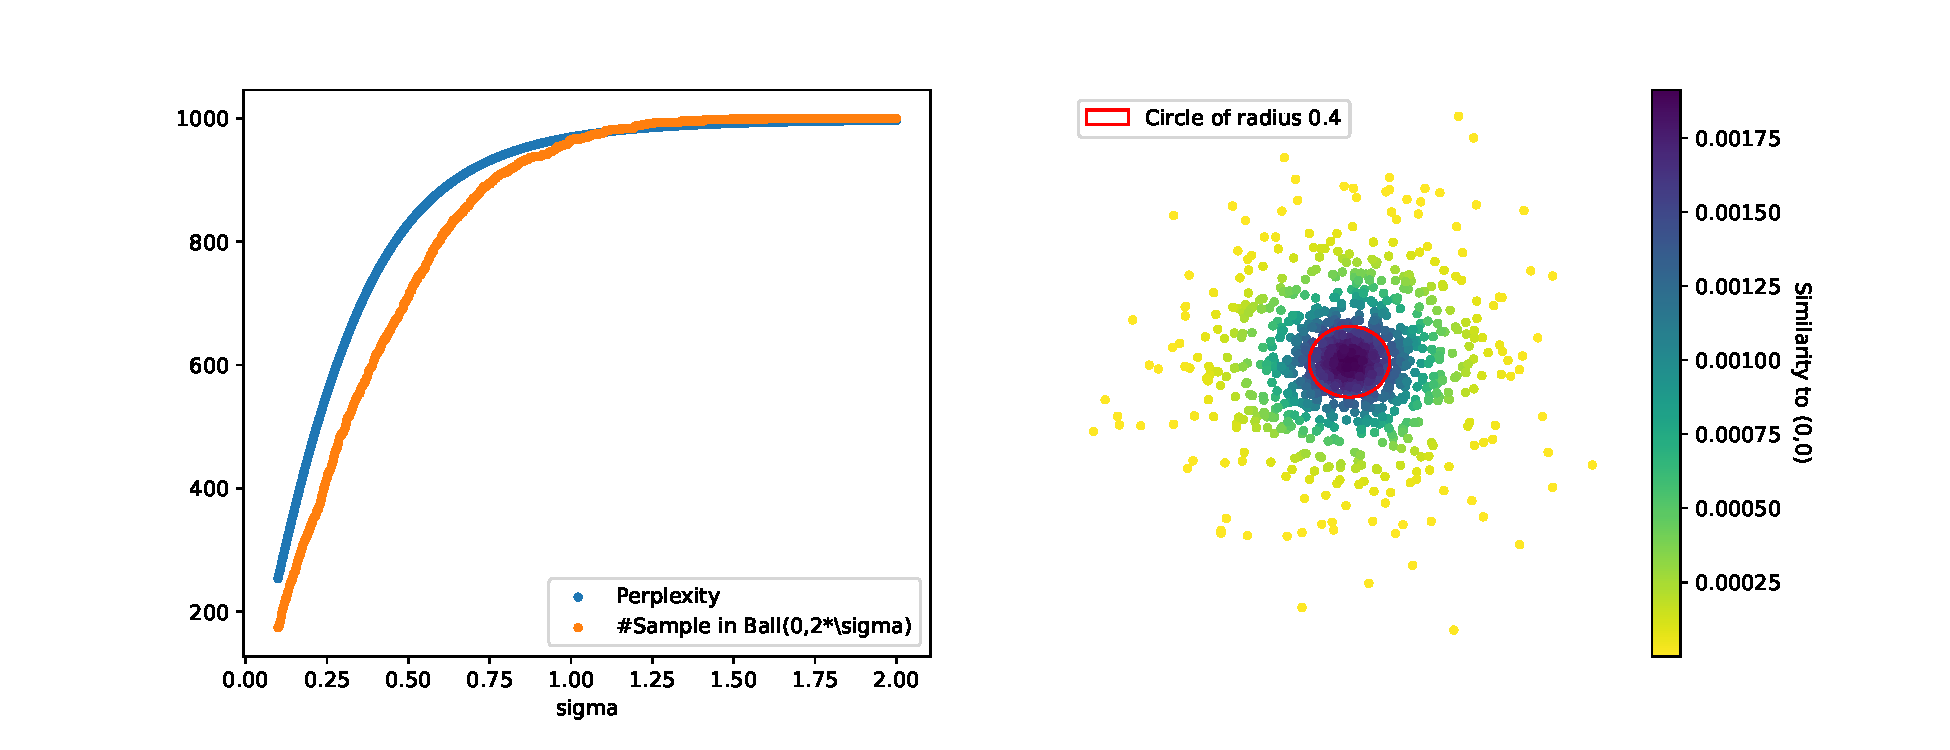
\includegraphics[clip, scale=0.32, trim=0 0 0
      1cm]{./pic/perplexity.pdf}
      \caption{Perplexity measures the number of samples in a
        neighborhood.\footnote{Original paper doesn't provide a proof, let us
      take it as an intuition.}}
    \end{figure}
  \end{minipage}
\end{frame}
\begin{frame}{Perplexity: Derivation of $\sigma$}
  \begin{obs}
    \vspace{1px}
    Perplexity of $\PP_i$ is continuous monotonic in $\sigma_i$.
  \end{obs}
  \vfill
  {\bf Binary Search:} Find $\sigma_i$ such that $Perp(\PP_i(\sigma_i))= K$\\
%  \begin{enumerate}
%    \item Fix a value $N_i$ of perplexity.
%    \item Initialize $\sigma_i^{(l)}$ such that $Perp(\PP_i)>N_i$
%    \item Initialize $\sigma_i^{(r)}$ such that $Perp(\PP_i)<N_i$
%    \item Until Convergence
%      \begin{itemize}
%        \item Compute the mean value $\bar{\sigma}$.
%        \item If $Perp(\PP_i(\bar{\sigma})>N_i$ then
%            $\sigma_i^{(r)}=\bar\sigma$
%        \item If $Perp(\PP_i(\bar{\sigma})<N_i$ then
%            $\sigma_i^{(l)}=\bar\sigma$
%      \end{itemize}
%  \end{enumerate}
  \begin{algorithm}[H]
    \SetKwInOut{Input}{input}\SetKwInOut{Output}{output}
    \SetAlgoLined
    $\sigma^{(l)}$ such that $Perp(\PP_i(\sigma^{(l)}))<K$\;
    $\sigma^{(r)}$ such that $Perp(\PP_i(\sigma^{(r)}))>K$\;
    \While{$|\sigma^{(r)} - \sigma^{(l)}| < \varepsilon$}{%
      $\bar\sigma\leftarrow (\sigma^{(l)} + \sigma^{(l)})/2$\;
      $p\leftarrow Perp(\PP_i(\bar\sigma))$\;
      \uIf{$p<K$}{%
        $\sigma^{(l)}\leftarrow\bar\sigma$;
      }
      \Else{%
        $\sigma^{(r)}\leftarrow\bar\sigma$;
      }
    }
    \Return{$\bar\sigma$}
  \end{algorithm}
\end{frame}
\section{t-SNE is t+SNE}
\begin{frame}{t-SNE: Symmetric + Student}
  In order to achieve better results Maaten \& Hinton modified SNE by
  \begin{enumerate}
    \item Using Student t-distribution for $\YY$
      \[
        \forall i,\quad
        q_{i|j} = \frac{(1+\|y_i-y_j\|^2)^{-1}}{\sum_{k\ne i}\left( 1+\|y_i +
        y_j\|^2\right)^{-1}},\quad \forall j\ne i
      \]
    \item Using symmetric versions of $p_{i|j},\,q_{i|j}$ by defining
      \[
        p_{ij}=\left( p_{i|j} + p_{j|i} \right)/(2n),\quad q_{ij}=\left(
        q_{i|j} + q_{j|i} \right)/(2n)
      \]
      so that $\PP = \left\{ p_{ij} \right\}$ and $\QQ=\left\{ q_{ij}
      \right\}$ are joint probabilities.
    \item The cost function becomes
      \[
        C(\YY) = KL(\PP,\QQ)
      \]
  \end{enumerate}
\end{frame}
\begin{frame}{t-SNE: Cost Interpretation}
  Let we consider a dummy case $\XX=\left\{ x_1,x_2 \right\}$. Then
  \begin{equation}
    \begin{aligned}
    \mbox{\bf SNE}\quad (\nabla C)_1 &=
      2(p_{1|2}+p_{2|1}-q_{1|2}-q_{2|1})(y_1-y_2)\\
      \mbox{\bf t-SNE}\quad (\nabla C )_1 &=
      4(p_{12}-q_{12})\left( y_1-y_2 \right)\left( 1+\|y_1 - y_2\|^2
      \right)^{-1}\\
    \end{aligned}
  \end{equation}
  {\bf Observation:} Both depends only on $\|x_1 -x_2\|$ and $\|y_1 -y_2\|$.
  \begin{figure}[h!]
    \centering
    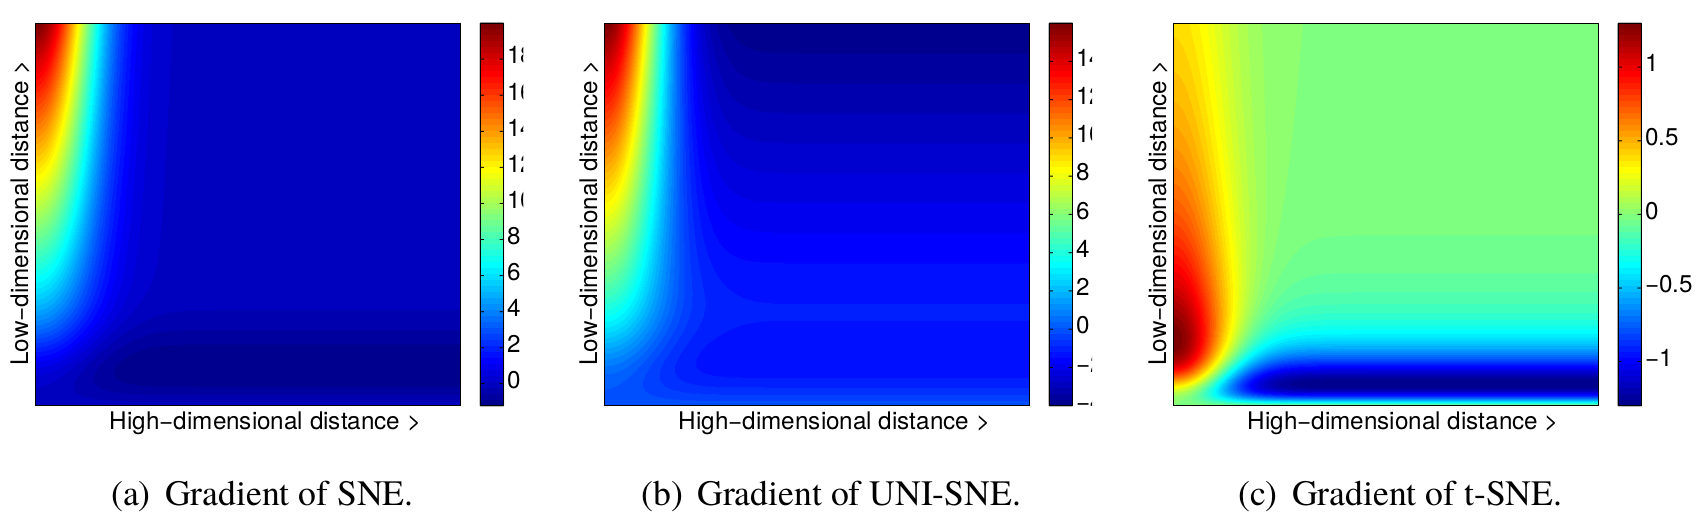
\includegraphics[scale=0.17]{./pic/gradient.png}
    \caption{Image taken from Maaten \& Hinton's paper representing $\|\nabla
      C\|$ for different distances in the input-space and in the embedding
    space.}
  \end{figure}
\end{frame}
\section{Examples}
\begin{frame}{t-SNE on cortex's cells}
  \begin{figure}[h!]
    \centering
    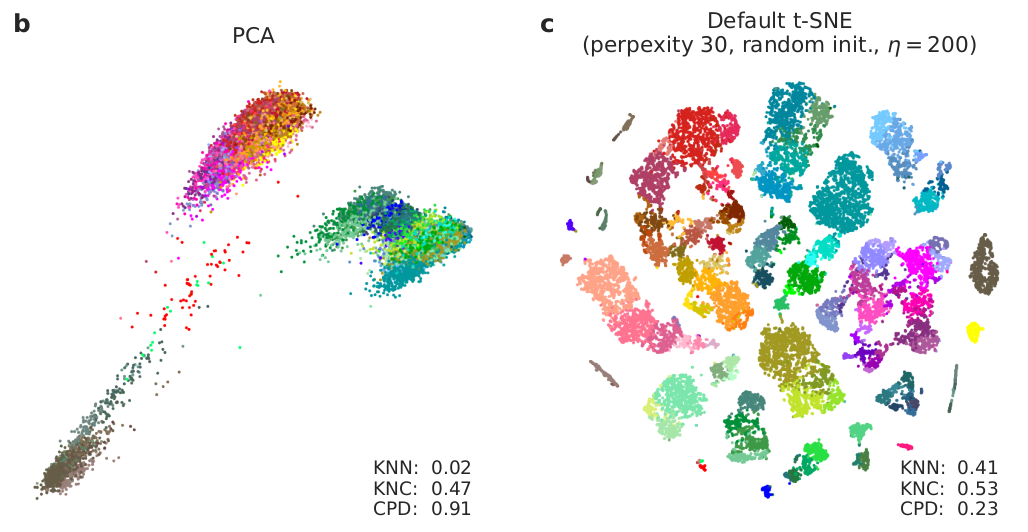
\includegraphics[scale=0.27]{./pic/cells.png}
    \caption{Image taken from Kobak-Barens paper.}
    \label{cortex}
  \end{figure}
  An hand made hierarchical clustering of cortex's cell is visualized
  through t-SNE\@. PCA is able to find the main three clusters but not to
  distinguish the sub-clusters.
\end{frame}
\begin{frame}{t-SNE on cortex' cells: Metrics Evaluations}
  \begin{itemize}
    \item {\bf KNN:} local metric. For each samples $x_i\in\XX$ and its
      image $y_i\in\YY$ we take the first k-closest points $K_i$ and $H_i$
      and we evaluate
      \[
        KNN := \frac{1}{|\XX|}\sum_i \frac{|H_i\cap \Phi(K_i)|}{k}
      \]
    \item {\bf KNC:} Cluster metric. The same as KNN but applied to
      $c_1,\cdots,c_s$ cluster's centroids.
    \item {\bf CPD:} Global metric. Defined as the Spearmen
      correlation.
  \end{itemize}
  These metrics in the figure~\ref{cortex} shows that t-SNE performs
  better in preserving local structures and worst in preserving the global
  structure of the data\footnote{Kobak-Barens paper for more details.}.
\end{frame}
\begin{frame}{t-SNE on MNIST}
  \begin{figure}[h!]
    \centering
    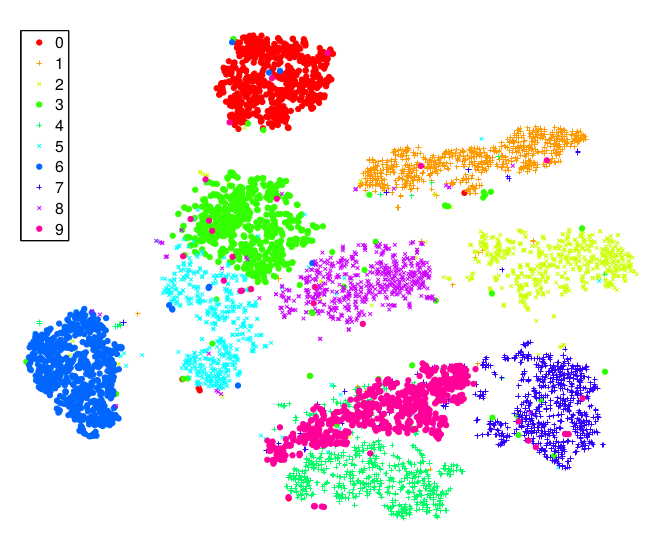
\includegraphics[scale=0.35]{./pic/MNIST.png}
    \caption{\vspace{1px} Image taken from Maaten - Hinton paper}
  \end{figure}
\end{frame}
\section{t-SNE Warnings}
\begin{frame}{How to use t-SNE\footnote{In this section we will show the results in
  \href{https://distill.pub/2016/misread-tsne}{\color{ggreen}Wattenberg -
online paper.}}}{}
\begin{center}
  \bf Hyper-Parameters really matter.
\end{center}
\begin{figure}[h!]
  \centering
  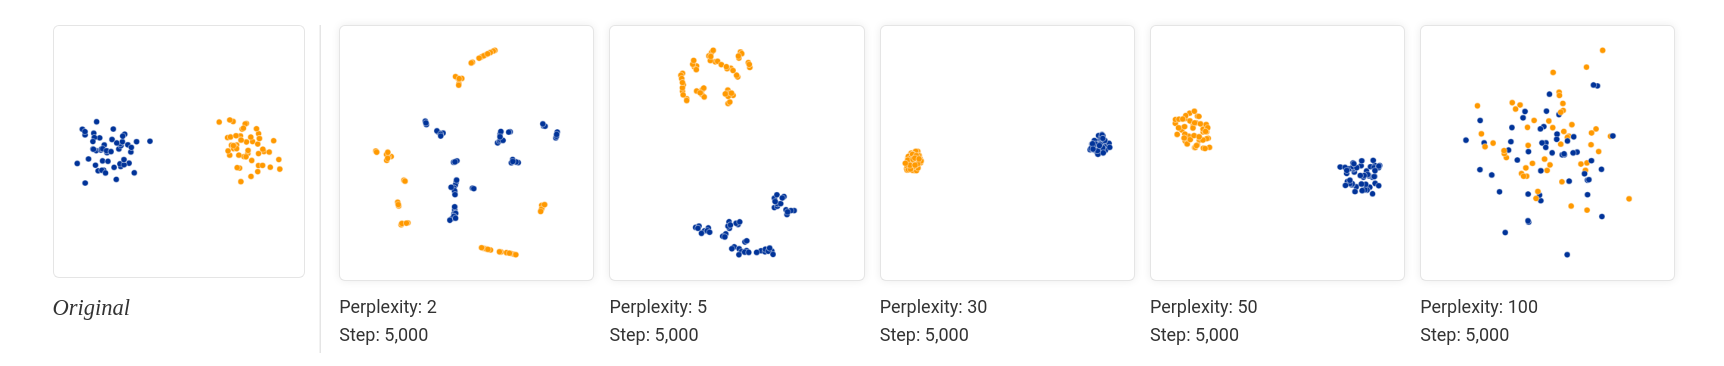
\includegraphics[scale=0.2, trim=3cm 0 0 0]{./pic/choose_perp.png}
\end{figure}
\begin{figure}[h!]
  \centering
  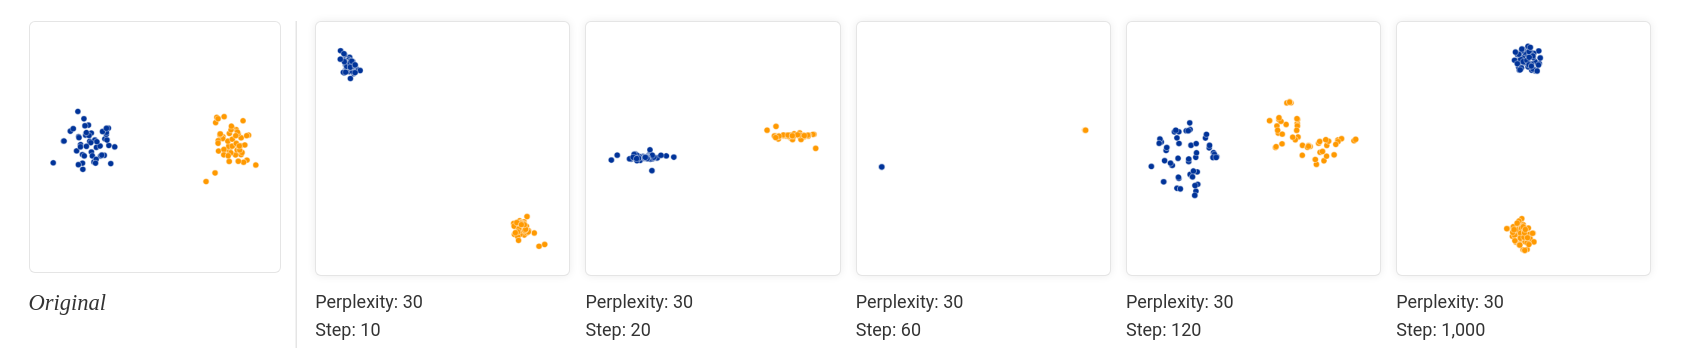
\includegraphics[scale=0.2, trim=2cm 0 0 3cm]{./pic/choose_steps.png}
\end{figure}
\hspace{3cm}
\end{frame}
\begin{frame}{How to use t-SNE}
  \begin{center}
    \bf
    Cluster sizes in a t-SNE plot has no meaning.
  \end{center}
  \begin{figure}[h]
    \centering
    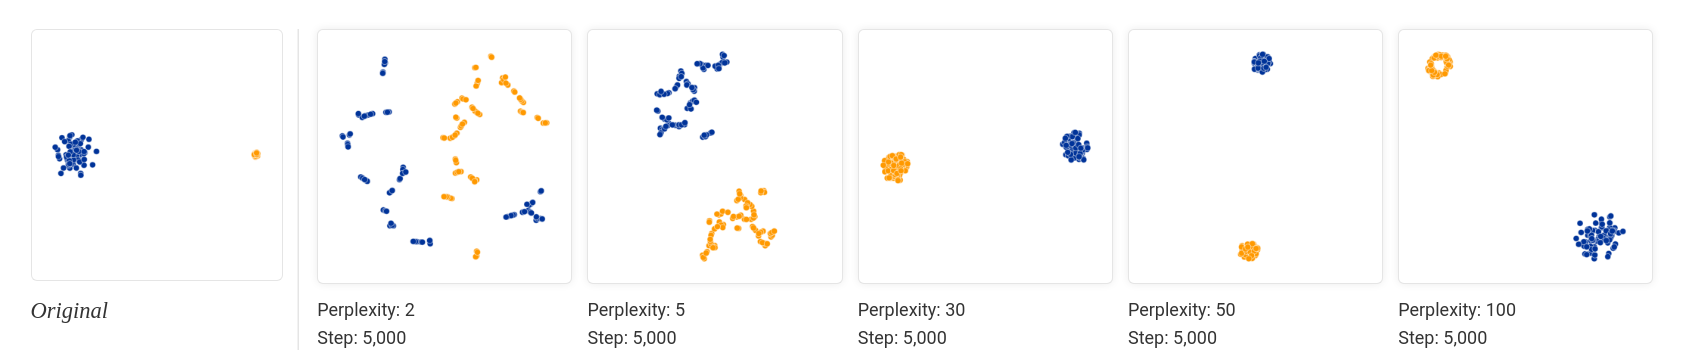
\includegraphics[scale=0.2, trim=2cm 0 0 0]{./pic/cluster_size.png}
  \end{figure}
\end{frame}
\begin{frame}{How to use t-SNE}
  \begin{center}
    \bf
    There is not control of the distances between clusters.
  \end{center}
  \begin{figure}[h]
    \centering
    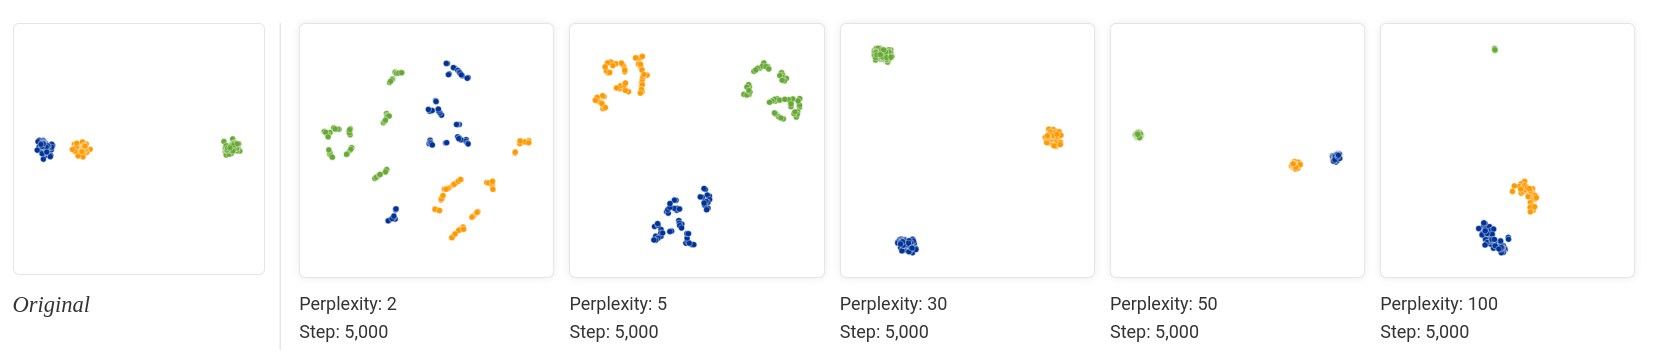
\includegraphics[scale=0.2, trim=2cm 0 0 2cm]{./pic/cluster_dist1.png}
  \end{figure}
  \begin{figure}[h]
    \centering
    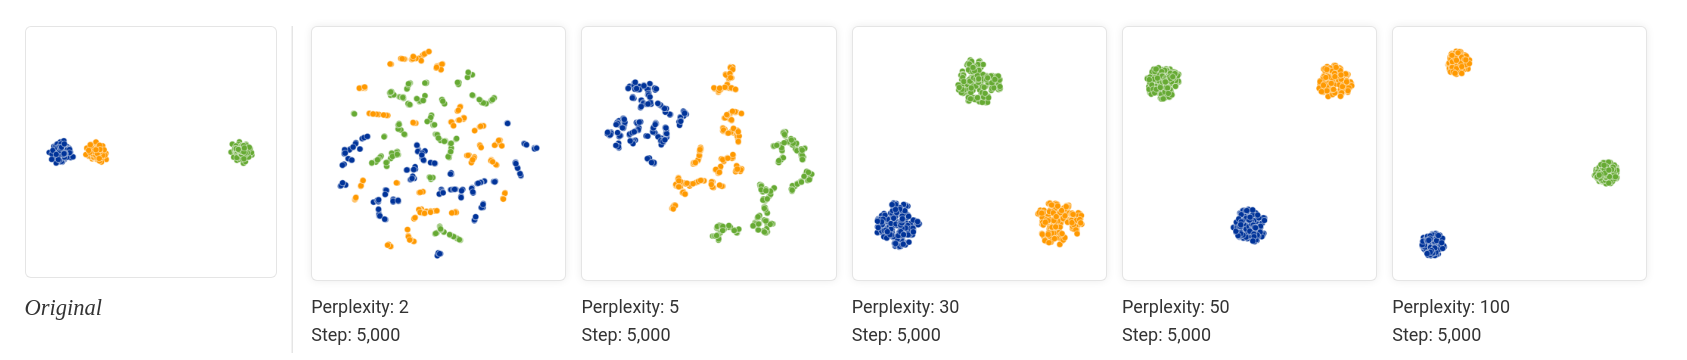
\includegraphics[scale=0.2, trim=2.3cm 0 0 3cm]{./pic/cluster_dist2.png}
  \end{figure}
  {\it Different initializations produce visualizations within clusters at
  different distances.}
\end{frame}
\begin{frame}{How to use t-SNE}
  \begin{center}
    \bf Sometimes topology is not preserved.
  \end{center}
  \begin{figure}[h!]
    \centering
    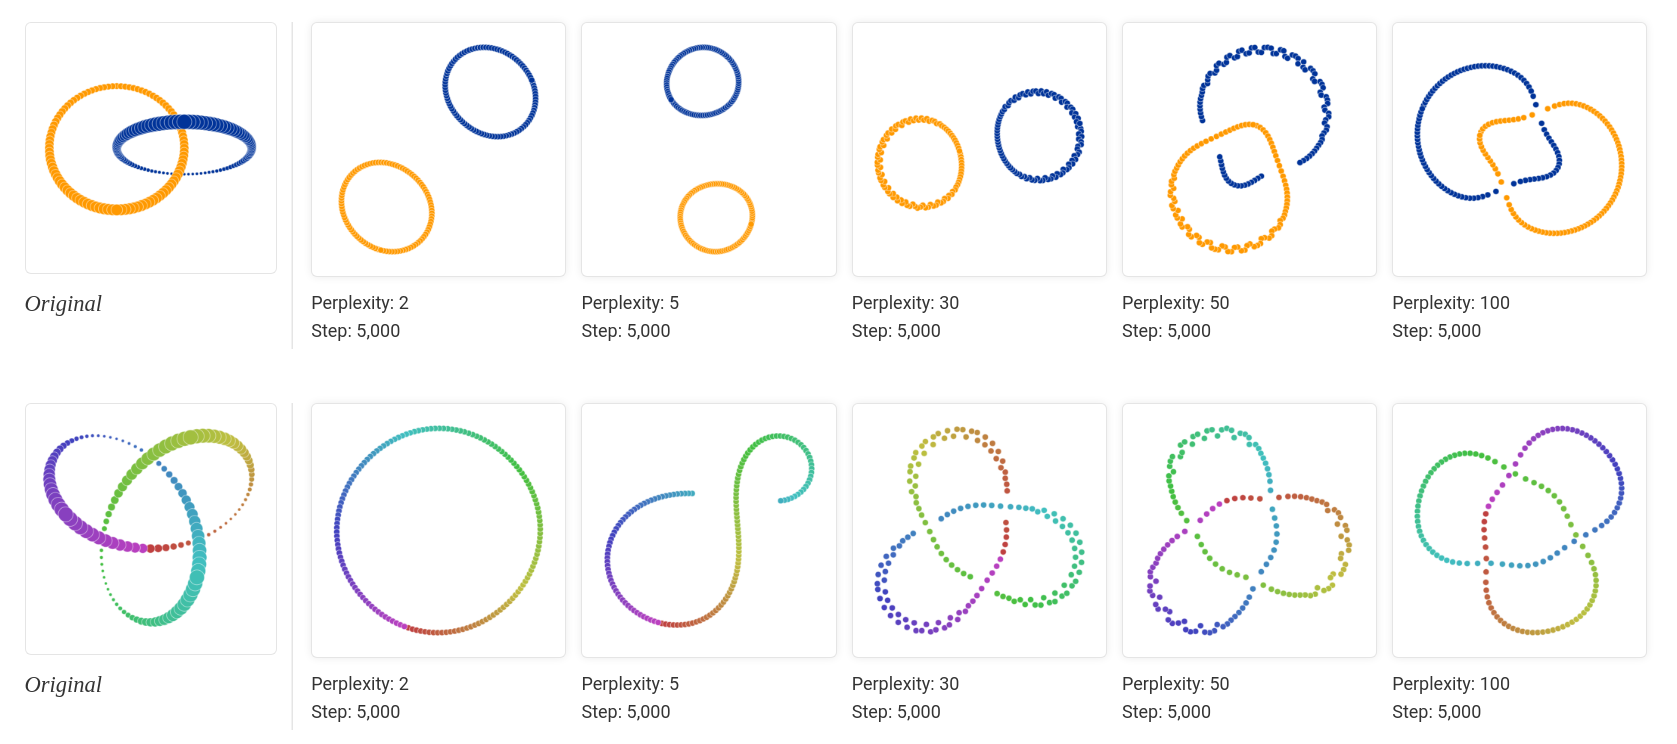
\includegraphics[scale=0.2, trim = 2cm 0 0 0]{pic/topology.png}
  \end{figure}
\end{frame}
\begin{frame}{Conclusion}
  \begin{minipage}{0.45\textwidth}
    \begin{center}
      {\bf What is t-SNE good for}
    \end{center}
    \begin{enumerate}
      \item Exploring data making associations based on geometrical
        informations in the original space.
      \item Providing intuition over the data that can be established  with different
        techniques.
    \end{enumerate}
  \end{minipage}
  \hfill
  \begin{minipage}[h!]{0.45\textwidth}
    \begin{center}
      {\bf How to not use t-SNE}
    \end{center}
    \vspace{.8cm}
    \begin{enumerate}
      \item To evaluate distances between clusters.
      \item To evaluate density of clusters.
      \item Establish topological property.
    \end{enumerate}
  \end{minipage}
\end{frame}
\begin{frame}{Conclusion}{}
    \begin{center}
       \Large
      Thanks for the attention.
    \end{center}
  \end{frame}
\end{document}

